% ============================================================
%  PRODUCT BREAKDOWN STRUCTURE (PBS) — Phase 1 : Démarrage
%  Time'Eats — Cellule PMO
%  Projet : Refonte Web
% ============================================================
\documentclass[11pt,a4paper,oneside]{report}
\usepackage{../../style/consulting}
\usepackage{pdflscape}
\hypersetup{pdftitle={PBS — Refonte Web — Time'Eats PMO}}
\pagestyle{fancy}\fancyhf{}
\renewcommand{\headrulewidth}{0pt}
\fancyhead[L]{\begin{tikzpicture}[remember picture,overlay]
  \draw[cnNavy,line width=0.5pt](0,0)--(\textwidth,0);
\end{tikzpicture}\vspace{2pt}\timeeatslogo\hspace{4pt}\small\textcolor{cnSlate}{Time'Eats \textbf{·} PBS --- \textit{Refonte Web}}}
\fancyhead[R]{\small\textcolor{cnSlate}{\thepage}}
\fancyfoot[C]{\tiny\textcolor{cnSlate}{Document confidentiel --- Cellule PMO --- CESI MAALSI 2026}}
\begin{document}\small

\begin{center}
{\LARGE\bfseries\color{cnNavy} Product Breakdown Structure (PBS)}\\[4pt]
\textcolor{cnOrange}{\rule{10cm}{1pt}}\\[4pt]
{\large\color{cnSlate} Phase 1 --- Démarrage \quad|\quad Projet : \textbf{Refonte Web}}
\end{center}

\vspace{6pt}
\renewcommand{\arraystretch}{1.4}
\begin{tabularx}{\textwidth}{L{3.5cm} Y L{3.5cm} Y}
\toprule
\rowcolor{cnNavy}\th{Projet} & \th{} & \th{Date} & \th{} \\
\midrule
Nom        & Refonte Web Time'Eats & Rédacteur & S. MARTIN (CP) \\
\rowcolor{cnIce}
Code       & RW-2026              & Version   & 1.0 (15/04/2026) \\
\bottomrule
\end{tabularx}

\section*{1 --- Objet du document}

Ce PBS décompose le produit \textbf{Refonte Web Time'Eats} en 7 sous-systèmes et 24 composants. Il sert de base au CDC (P1-02ter), au WBS (P2-06) et au budget (P2-08). Il reflète le périmètre \textit{Inclus} défini dans la Note de cadrage (P1-02) et le PMP (P2-05 §2).

\section*{2 --- Vue arborescente synthétique}

Le diagramme page suivante (généré depuis \texttt{pbs\_refonte\_web.puml} via PlantUML) présente la décomposition produit à 3 niveaux : Produit $\to$ Sous-systèmes $\to$ Composants. La page est en orientation paysage pour préserver la lisibilité des 24 composants.

\begin{landscape}
\thispagestyle{empty}
\vspace*{\fill}
\begin{center}
{\large\bfseries\color{cnNavy} PBS --- Refonte Web Time'Eats (RW-2026)}\\[6pt]
\textcolor{cnOrange}{\rule{14cm}{0.8pt}}\\[10pt]
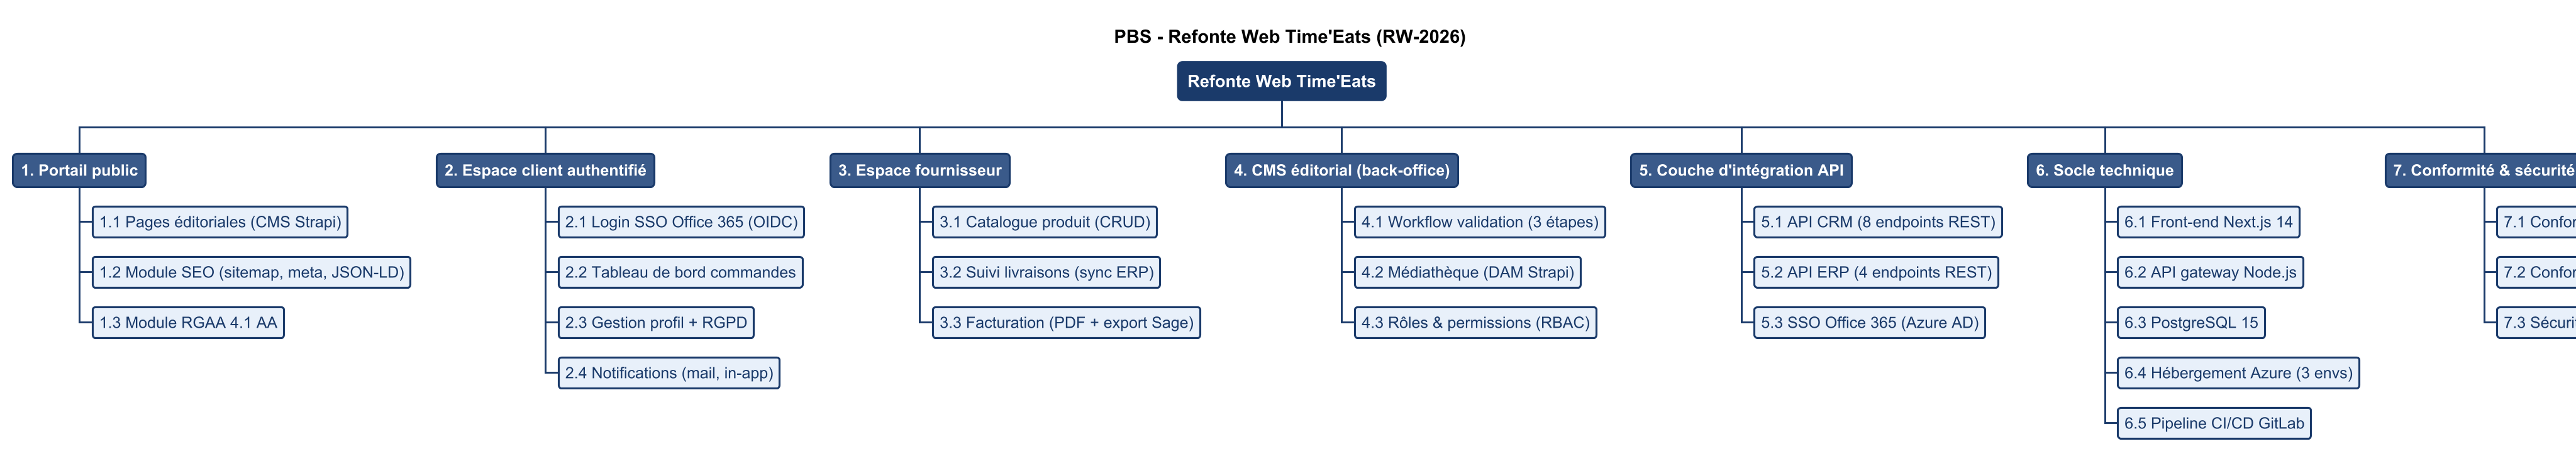
\includegraphics[width=\linewidth,keepaspectratio]{../../diagrammes/pbs_refonte_web.png}\\[8pt]
{\footnotesize Source : \texttt{pbs\_refonte\_web.puml} --- régénération : \texttt{plantuml pbs\_refonte\_web.puml}.}
\end{center}
\vspace*{\fill}
\end{landscape}

\section*{3 --- Décomposition détaillée (niveau 3)}

\renewcommand{\arraystretch}{1.3}
\begin{tabularx}{\textwidth}{C{1cm} L{3.7cm} L{3.8cm} Y}
\toprule
\rowcolor{cnNavy}\th{Code} & \th{Sous-système} & \th{Composant} & \th{Éléments / contenu} \\
\midrule
1   & \textbf{Portail public} & & Visiteurs anonymes, ~50k visites/mois cible \\
\rowcolor{cnIce}
1.1 & & Pages éditoriales (CMS) & 12 templates : accueil, offre B2B, offre B2C, presse, recrutement, blog, contact, mentions légales, RGPD, cookies, accessibilité, plan du site \\
1.2 & & Module SEO              & Sitemap XML auto, balises meta dynamiques, JSON-LD (Organization, Article, FAQ), redirections 301 depuis ancien site \\
\rowcolor{cnIce}
1.3 & & Module RGAA             & Skip links, contraste $\geq$ 4.5:1, focus visible, navigation clavier, attributs ARIA, déclaration d'accessibilité \\
\midrule
2   & \textbf{Espace client} & & Clients B2B et B2C authentifiés \\
\rowcolor{cnIce}
2.1 & & Login SSO Office 365 (OIDC) & Authentification via Azure AD, MFA optionnelle, refresh token, logout SSO \\
2.2 & & Tableau de bord commandes   & Historique commandes 24 mois, suivi en cours, téléchargement factures PDF, réabonnement 1-clic \\
\rowcolor{cnIce}
2.3 & & Gestion profil + RGPD       & Édition coordonnées, préférences notifications, export données personnelles (JSON), suppression compte \\
2.4 & & Notifications               & Templates mail (SendGrid), in-app (websocket), préférences par canal \\
\midrule
3   & \textbf{Espace fournisseur} & & Restaurateurs / traiteurs partenaires \\
\rowcolor{cnIce}
3.1 & & Catalogue produit (CRUD) & Création / édition / désactivation produit, photos (max 5), allergènes, prix HT/TTC, stock indicatif \\
3.2 & & Suivi livraisons          & Synchro temps réel avec ERP (statut Préparation / Expédié / Livré), preuve de livraison PDF \\
\rowcolor{cnIce}
3.3 & & Facturation               & Génération automatique facture mensuelle PDF, export comptable CSV, relances automatiques J+30 \\
\midrule
4   & \textbf{CMS éditorial} & & Équipe marketing (4 personnes) \\
\rowcolor{cnIce}
4.1 & & Workflow validation & Brouillon $\to$ Relecture $\to$ Publication, notification email, historique versions (10 dernières) \\
4.2 & & Médiathèque (DAM)   & Strapi assets, ré-encodage automatique (WebP, AVIF), 3 tailles responsives, recherche full-text \\
\rowcolor{cnIce}
4.3 & & Rôles / permissions & 4 rôles : Rédacteur, Relecteur, Administrateur, Super-admin (RBAC) \\
\midrule
5   & \textbf{Couche API} & & Interopérabilité avec SI Time'Eats \\
\rowcolor{cnIce}
5.1 & & API CRM   & 8 endpoints REST JSON : GET/POST comptes, GET/POST contacts, GET opportunités, POST leads, GET catalogue, POST commande \\
5.2 & & API ERP   & 4 endpoints REST : GET produits, GET stocks, POST factures, GET statut livraison \\
\rowcolor{cnIce}
5.3 & & SSO Azure AD & OIDC, scopes openid profile email, app registration Azure AD, certificats \\
\midrule
6   & \textbf{Socle technique} & & Stack et infrastructure \\
\rowcolor{cnIce}
6.1 & & Front-end Next.js 14   & SSR, ISR pour pages CMS, App Router, Tailwind CSS, TypeScript strict \\
6.2 & & API gateway Node.js    & Express 4, validation Zod, rate limiting, JWT validation, logs structurés \\
\rowcolor{cnIce}
6.3 & & PostgreSQL 15          & 32 tables, migrations Prisma, RGPD : anonymisation J+1825 \\
6.4 & & Hébergement Azure      & 3 environnements (dev / staging / prod), région West Europe, App Service P1v3, sauvegardes quotidiennes 30 j \\
\rowcolor{cnIce}
6.5 & & Pipeline CI/CD GitLab  & Lint, tests unitaires, build, déploiement auto staging, déploiement manuel prod, scan SAST (SonarQube), scan dépendances (Trivy) \\
\midrule
7   & \textbf{Conformité \& sécurité} & & Obligations légales et standards \\
\rowcolor{cnIce}
7.1 & & Conformité RGPD       & Registre traitements, mentions légales, bandeau cookies (Axeptio), DPO référent, PIA si besoin \\
7.2 & & Conformité RGAA 4.1 AA & Audit externe par bureau spécialisé, $\geq 95\,\%$ critères conformes, déclaration publique \\
\rowcolor{cnIce}
7.3 & & Sécurité OWASP ASVS L2 & Pentest pré go-live, 0 vulnérabilité critique, headers sécurité (CSP, HSTS, X-Frame-Options), secrets dans Azure Key Vault \\
\bottomrule
\end{tabularx}

\section*{4 --- Correspondance PBS $\leftrightarrow$ autres documents}

\renewcommand{\arraystretch}{1.3}
\begin{tabularx}{\textwidth}{L{3cm} L{3cm} Y}
\toprule
\rowcolor{cnNavy}\th{Sous-système PBS} & \th{Lots WBS (P2-06)} & \th{Exigences CDC (P1-02ter)} \\
\midrule
1. Portail public    & WP-3, WP-4         & FX-01 à FX-05, NFX-01 (perf), NFX-02 (RGAA) \\
\rowcolor{cnIce}
2. Espace client     & WP-5, WP-6         & FX-06 à FX-10, NFX-03 (SSO) \\
3. Espace fournisseur& WP-7               & FX-11 à FX-13 \\
\rowcolor{cnIce}
4. CMS éditorial     & WP-8               & FX-14 à FX-16 \\
5. Couche API        & WP-9, WP-10        & FX-17, FX-18, NFX-04 (contrats API) \\
\rowcolor{cnIce}
6. Socle technique   & WP-1, WP-2, WP-11  & NFX-05 (perf), NFX-06 (dispo), NFX-07 (compat) \\
7. Conformité \& sécu & WP-12             & FX-19, FX-20, NFX-08 à NFX-10 \\
\bottomrule
\end{tabularx}

\begin{reco}
\textbf{Périmètre stable au J0 (kick-off, 22/04/2026)} --- toute évolution du PBS (ajout / suppression de composant) doit faire l'objet d'une demande de changement formelle (P3-14) impactant le baseline scope / coût / délai. La couche \textbf{App mobile clients / fournisseurs} \emph{n'est pas} dans ce PBS : projets dédiés du portefeuille (cf.\ §1.5 du livrable PMO).
\end{reco}

\end{document}
